\documentclass[11pt, letterpaper]{article}

% ── Geometry & Layout ──
\usepackage[margin=1in]{geometry}
\usepackage{parskip}
\usepackage{enumitem}
\usepackage{titlesec}
\usepackage{fancyhdr}
\usepackage{lastpage}

% ── Fonts & Encoding ──
\usepackage[T1]{fontenc}
\usepackage[utf8]{inputenc}
\usepackage{libertine}
\usepackage[libertine]{newtxmath}
\usepackage{inconsolata}

% ── Color & Graphics ──
\usepackage[dvipsnames,svgnames,x11names]{xcolor}
\usepackage{tikz}
\usetikzlibrary{
  positioning, arrows.meta, calc, backgrounds,
  fit, decorations.pathreplacing, shapes.geometric,
  patterns, shadows
}
\usepackage{graphicx}

% ── Tables ──
\usepackage{booktabs}
\usepackage{tabularx}
\usepackage{multirow}
\usepackage{array}
\newcolumntype{L}[1]{>{\raggedright\arraybackslash}p{#1}}
\newcolumntype{C}[1]{>{\centering\arraybackslash}p{#1}}

% ── Code & Math ──
\usepackage{listings}
\usepackage{amsmath}

% ── Hyperlinks ──
\usepackage[colorlinks=true, linkcolor=NavyBlue, urlcolor=NavyBlue, citecolor=NavyBlue]{hyperref}

% ── Section Formatting ──
\titleformat{\section}{\Large\bfseries\color{NavyBlue}}{\thesection}{1em}{}[\vspace{-0.3em}\textcolor{NavyBlue!30}{\rule{\textwidth}{0.8pt}}]
\titleformat{\subsection}{\large\bfseries\color{NavyBlue!80}}{\thesubsection}{0.8em}{}
\titleformat{\subsubsection}{\normalsize\bfseries\color{NavyBlue!60}}{\thesubsubsection}{0.6em}{}

% ── Header/Footer ──
\pagestyle{fancy}
\fancyhf{}
\renewcommand{\headrulewidth}{0.4pt}
\fancyhead[L]{\small\textcolor{gray}{Cross-Patient uECOG Speech Decoding}}
\fancyhead[R]{\small\textcolor{gray}{Tang \& Spalding --- March 2026}}
\fancyfoot[C]{\small\textcolor{gray}{Page \thepage\ of \pageref{LastPage}}}

% ── Code Listing Style ──
\lstset{
  basicstyle=\ttfamily\small,
  backgroundcolor=\color{gray!6},
  frame=single,
  framerule=0.4pt,
  rulecolor=\color{gray!40},
  breaklines=true,
  columns=fullflexible,
  keepspaces=true,
  xleftmargin=1em,
  xrightmargin=1em,
  aboveskip=0.8em,
  belowskip=0.8em,
}

% ── Custom Colors ──
\definecolor{cInput}{HTML}{4A90D9}
\definecolor{cPerPt}{HTML}{F5A623}
\definecolor{cShared}{HTML}{50B860}
\definecolor{cSharedDk}{HTML}{2E7D32}
\definecolor{cLoss}{HTML}{E74C3C}
\definecolor{cLossDk}{HTML}{C62828}
\definecolor{cInnov}{HTML}{8E24AA}
\definecolor{cInnovLt}{HTML}{CE93D8}
\definecolor{cStat}{HTML}{90A4AE}
\definecolor{cNote}{HTML}{FFF8E1}
\definecolor{cNoteBd}{HTML}{FFE082}

% ── TikZ Styles ──
\tikzset{
  block/.style={
    rectangle, rounded corners=5pt, minimum width=10cm, minimum height=1.2cm,
    text=white, font=\sffamily\bfseries, align=center,
    drop shadow={shadow xshift=0.5pt, shadow yshift=-1pt, opacity=0.15}
  },
  smallblock/.style={
    rectangle, rounded corners=4pt, minimum width=8cm, minimum height=1cm,
    text=white, font=\sffamily\small\bfseries, align=center,
    drop shadow={shadow xshift=0.5pt, shadow yshift=-1pt, opacity=0.12}
  },
  note/.style={
    rectangle, rounded corners=3pt, fill=gray!8, draw=gray!30,
    font=\sffamily\footnotesize, align=left, text width=4.5cm, inner sep=5pt
  },
  annotate/.style={
    rectangle, rounded corners=3pt, font=\sffamily\scriptsize,
    align=center, inner sep=4pt
  },
  arrow/.style={-{Stealth[length=5pt]}, thick, color=gray!70},
  thinarrow/.style={-{Stealth[length=4pt]}, color=gray!60},
  zone/.style={
    rectangle, rounded corners=8pt, draw=#1, line width=1.2pt,
    inner sep=8pt
  },
  badge/.style={
    rectangle, rounded corners=8pt, fill=#1, text=white,
    font=\sffamily\scriptsize\bfseries, inner sep=3pt
  },
}

\begin{document}

% ══════════════════════════════════════════════════════════════
% TITLE PAGE
% ══════════════════════════════════════════════════════════════

\thispagestyle{empty}
\begin{center}
\vspace*{2cm}

{\Huge\bfseries\color{NavyBlue} Cross-Patient Speech Decoding\\[6pt] from Intra-Operative \textmu ECoG}

\vspace{1.2cm}
{\Large Technical Memo: Research Plan}

\vspace{1.5cm}
\textcolor{gray!60}{\rule{12cm}{0.8pt}}
\vspace{1cm}

{\large
\textbf{Ben Tang}\\[4pt]
Greg Cogan Lab, Duke University\\[12pt]
\textbf{Collaborator:} Zac Spalding
}

\vspace{1cm}
{\large March 17, 2026}

\vspace{2cm}
\begin{minipage}{13cm}
\textcolor{gray!80}{\itshape
Synthesizes 18 papers on cross-patient neural speech decoding into a two-phase implementation plan. Phase~2 modernizes Spalding's PCA+CCA+SVM to the field-standard end-to-end pipeline. Phase~3 introduces two architectural innovations---each absent from the neural speech BCI field---while keeping training field-standard.}
\end{minipage}

\vfill
\textcolor{gray!40}{\small Supporting files:
\texttt{implementation\_plan.md} $\cdot$
\texttt{research\_synthesis.md} $\cdot$
\texttt{future\_directions.md}}
\end{center}

\newpage
\setcounter{page}{1}

% ══════════════════════════════════════════════════════════════
\tableofcontents
\newpage

% ══════════════════════════════════════════════════════════════
\section{Summary}
% ══════════════════════════════════════════════════════════════

I have reviewed 18 papers on cross-patient neural speech decoding and designed a two-phase plan to replace the PCA+CCA+SVM pipeline (0.31 bal acc) with the modern field-standard architecture, then add two novel architectural innovations. The plan is conservative: 8 of 10 pipeline components are field-standard with multi-paper support. The 2 novel components are independently ablated.

\textbf{Bottom line:} Phase~2 (field standard) is a guaranteed improvement. Phase~3 adds two architectural ideas absent from the field---per-patient spatial conv and an articulatory decomposition CTC head. Training is identical in both phases (standard multi-patient SGD, same as Singh 2025).

\subsection{Papers Reviewed}

Spalding 2025, Duraivel 2023/2025, Singh 2025, Boccato 2026, Levin 2026, BIT (Zhang 2026), wav2vec ECoG 2024, Dual Pathway 2025, Chen 2024, Chen 2025 (SwinTW), MIBRAIN 2025, Wu 2025, Willett 2023, Metzger 2023, Littlejohn 2025, Nason 2026, Qian 2025.


% ══════════════════════════════════════════════════════════════
\section{What the Literature Tells Us}
\label{sec:lit}
% ══════════════════════════════════════════════════════════════

\subsection{Architecture Consensus}

Every successful cross-patient speech BCI from the last two years uses:

\begin{center}
\fbox{\textbf{Per-patient input layer}\ $\longrightarrow$\ \textbf{Shared recurrent backbone}\ $\longrightarrow$\ \textbf{CTC/sequence loss}}
\end{center}

Used by Willett 2023, Metzger 2023, Boccato 2026, Levin 2026, Nason 2026, Singh 2025 (all GRU/LSTM + CTC). Littlejohn 2025 evolves this to RNN-T for streaming. BIT 2026 uses a transformer backbone + CTC but the same per-patient read-in pattern. The per-patient layer absorbs cross-patient variation; the shared backbone learns patient-invariant temporal dynamics; CTC handles variable-length alignment.

\subsection{Key Findings}

\textbf{Singh 2025} --- closest precedent. 25 sEEG patients, per-patient Conv1D, shared BiLSTM $2\times64$, CTC. Group PER 0.49 vs single 0.57 (${\sim}$14\% relative improvement). Only 2 layers of hidden size 64 for 36 phonemes (of 44 English)---our 9-phoneme task is far simpler.

\textbf{Boccato 2026} --- learned affine transforms are predominantly diagonal (per-channel gain). \textbf{Caveat:} this is Utah-specific (fixed stereotactic placement, same orientation). uECOG has variable surgical placement/orientation $\to$ cross-patient variation includes \emph{spatial remapping}, not just gain. This strengthens the case for spatial conv over linear read-in.

\textbf{Levin 2026} --- per-patient input layers are essential (shared input makes transfer \emph{worse}). 30\% source replay during fine-tuning prevents catastrophic forgetting.

\textbf{BIT (Zhang 2026)} --- SSL $\approx$ supervised for same-subject (Table~9). SSL advantage is cross-subject only. Supervised cross-patient with per-patient layers (Singh) works at our scale.

\textbf{Metzger 2023 / Littlejohn 2025} (Chang lab) --- Conv1d $\to$ GRU on 253-ch ECoG. Metzger: 4-layer BiGRU H=500, CTC, 50~Hz effective rate. Littlejohn: 3-layer uniGRU H=512, RNN-T (not CTC) for streaming at 12.5~Hz. N=1 (no cross-patient). Most systems use 12--20~Hz; Metzger's 50~Hz is the outlier (paired with much larger GRU). Supports our configurable downsampling.

\textbf{Wu 2025} --- articulatory features ``more robustly encoded in vSMC than acoustic features, learned faster with limited data.'' P3 was intra-operative (PCC=0.76)---closest analogue to our setting.

\subsection{What Doesn't Apply}

\begin{itemize}[nosep]
  \item \textbf{Spike-based FMs} (BIT 367~hrs, NDT3 2000~hrs): Poisson spikes $\neq$ Gaussian HGA
  \item \textbf{Large-scale SSL}: We have ${\sim}$3~hrs pooled; minimum successful SSL was ${\sim}$30~min/pt
  \item \textbf{Dual Pathway speech FM}: Validated for auditory cortex (STG) only
\end{itemize}


% ══════════════════════════════════════════════════════════════
\section{Architecture}
\label{sec:arch}
% ══════════════════════════════════════════════════════════════

\subsection{Phase 2: Field Standard (E1)}

\begin{figure}[h]
\centering
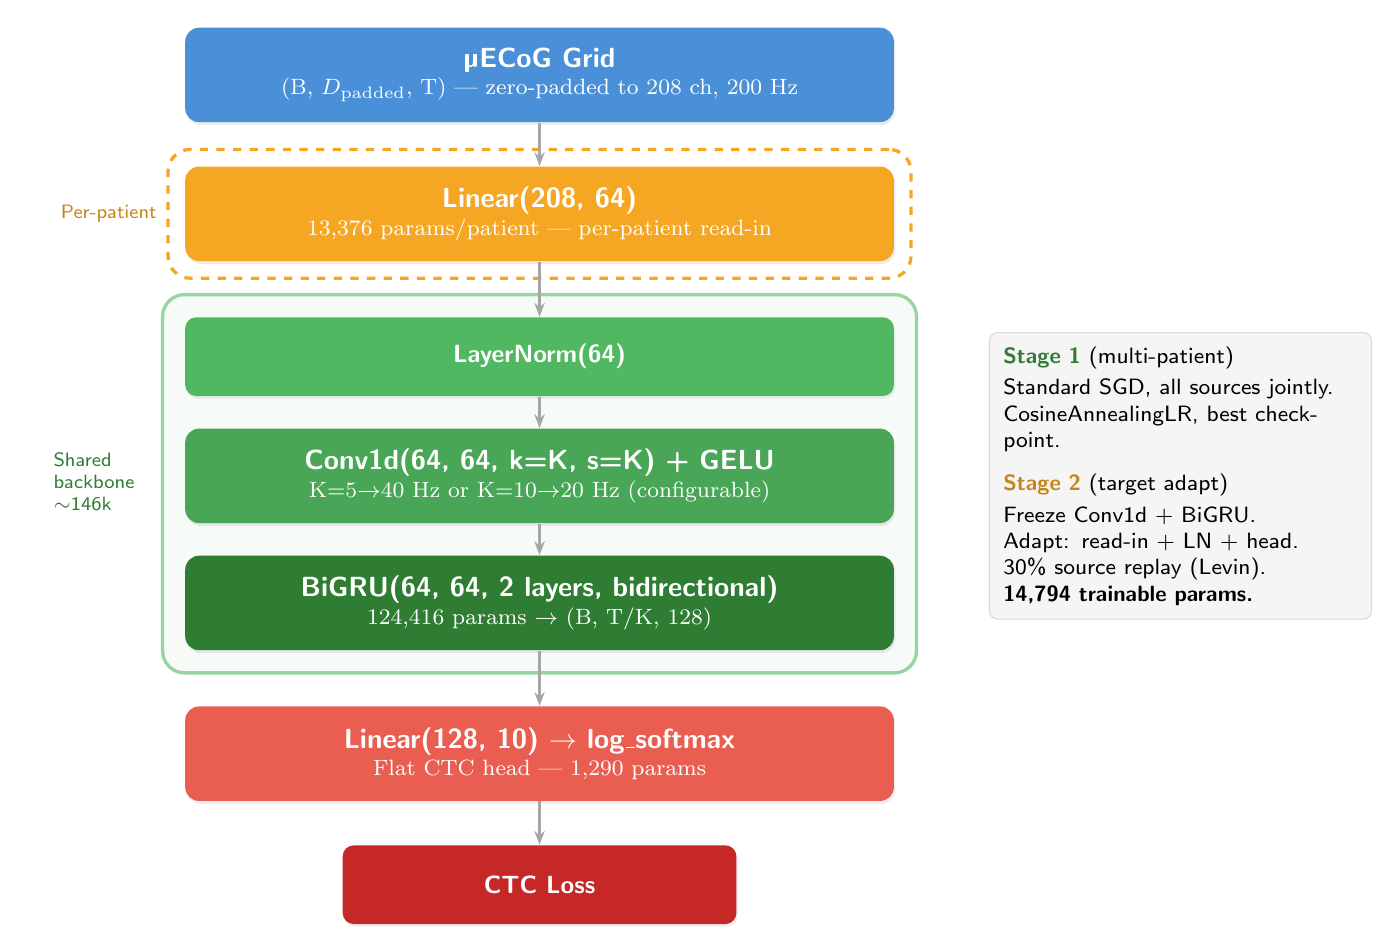
\begin{tikzpicture}[node distance=0.55cm]

  \node[block, fill=cInput, minimum width=9cm] (input)
    {\textmu ECoG Grid\\[-2pt]{\footnotesize\normalfont (B, $D_\text{padded}$, T) --- zero-padded to 208~ch, 200~Hz}};

  \node[block, fill=cPerPt, minimum width=9cm, below=of input] (readin)
    {Linear(208, 64)\\[-2pt]{\footnotesize\normalfont 13{,}376 params/patient --- per-patient read-in}};

  \node[smallblock, fill=cShared, minimum width=9cm, below=0.7cm of readin] (ln)
    {LayerNorm(64)};

  \node[block, fill=cShared!90!black, minimum width=9cm, below=0.4cm of ln] (conv)
    {Conv1d(64, 64, k=K, s=K) + GELU\\[-2pt]{\footnotesize\normalfont K=5$\to$40~Hz or K=10$\to$20~Hz (configurable)}};

  \node[block, fill=cSharedDk, minimum width=9cm, below=0.4cm of conv] (gru)
    {BiGRU(64, 64, 2 layers, bidirectional)\\[-2pt]{\footnotesize\normalfont 124{,}416 params $\to$ (B, T/K, 128)}};

  \node[block, fill=cLoss!90, minimum width=9cm, below=0.7cm of gru] (head)
    {Linear(128, 10) $\to$ log\_softmax\\[-2pt]{\footnotesize\normalfont Flat CTC head --- 1{,}290 params}};

  \node[smallblock, fill=cLossDk, minimum width=5cm, below=of head] (loss)
    {CTC Loss};

  \draw[arrow] (input)  -- (readin);
  \draw[arrow] (readin) -- (ln);
  \draw[arrow] (ln)     -- (conv);
  \draw[arrow] (conv)   -- (gru);
  \draw[arrow] (gru)    -- (head);
  \draw[arrow] (head)   -- (loss);

  \begin{scope}[on background layer]
    \node[zone=cPerPt, dashed, fit=(readin), inner sep=6pt,
          label={[font=\sffamily\scriptsize\color{cPerPt!80!black}]left:Per-patient}] {};
    \node[zone=cShared!60, fill=cShared!5, fit=(ln)(conv)(gru), inner sep=8pt,
          label={[font=\sffamily\scriptsize\color{cSharedDk}]left:\begin{tabular}{l}Shared\\backbone\\$\sim$146k\end{tabular}}] {};
  \end{scope}

  \node[note, right=1.2cm of conv] (tnote) {
    \textcolor{cSharedDk}{\textbf{Stage 1}} (multi-patient)\\[2pt]
    Standard SGD, all sources jointly.\\
    CosineAnnealingLR, best checkpoint.\\[6pt]
    \textcolor{cPerPt!80!black}{\textbf{Stage 2}} (target adapt)\\[2pt]
    Freeze Conv1d + BiGRU.\\
    Adapt: read-in + LN + head.\\
    30\% source replay (Levin).\\
    \textbf{14{,}794 trainable params.}
  };

\end{tikzpicture}
\caption{Phase~2 field standard (E1). Training identical to Phase~3.}
\label{fig:phase2}
\end{figure}


\subsection{Phase 3: Two Innovations (E2)}

\begin{figure}[h!]
\centering
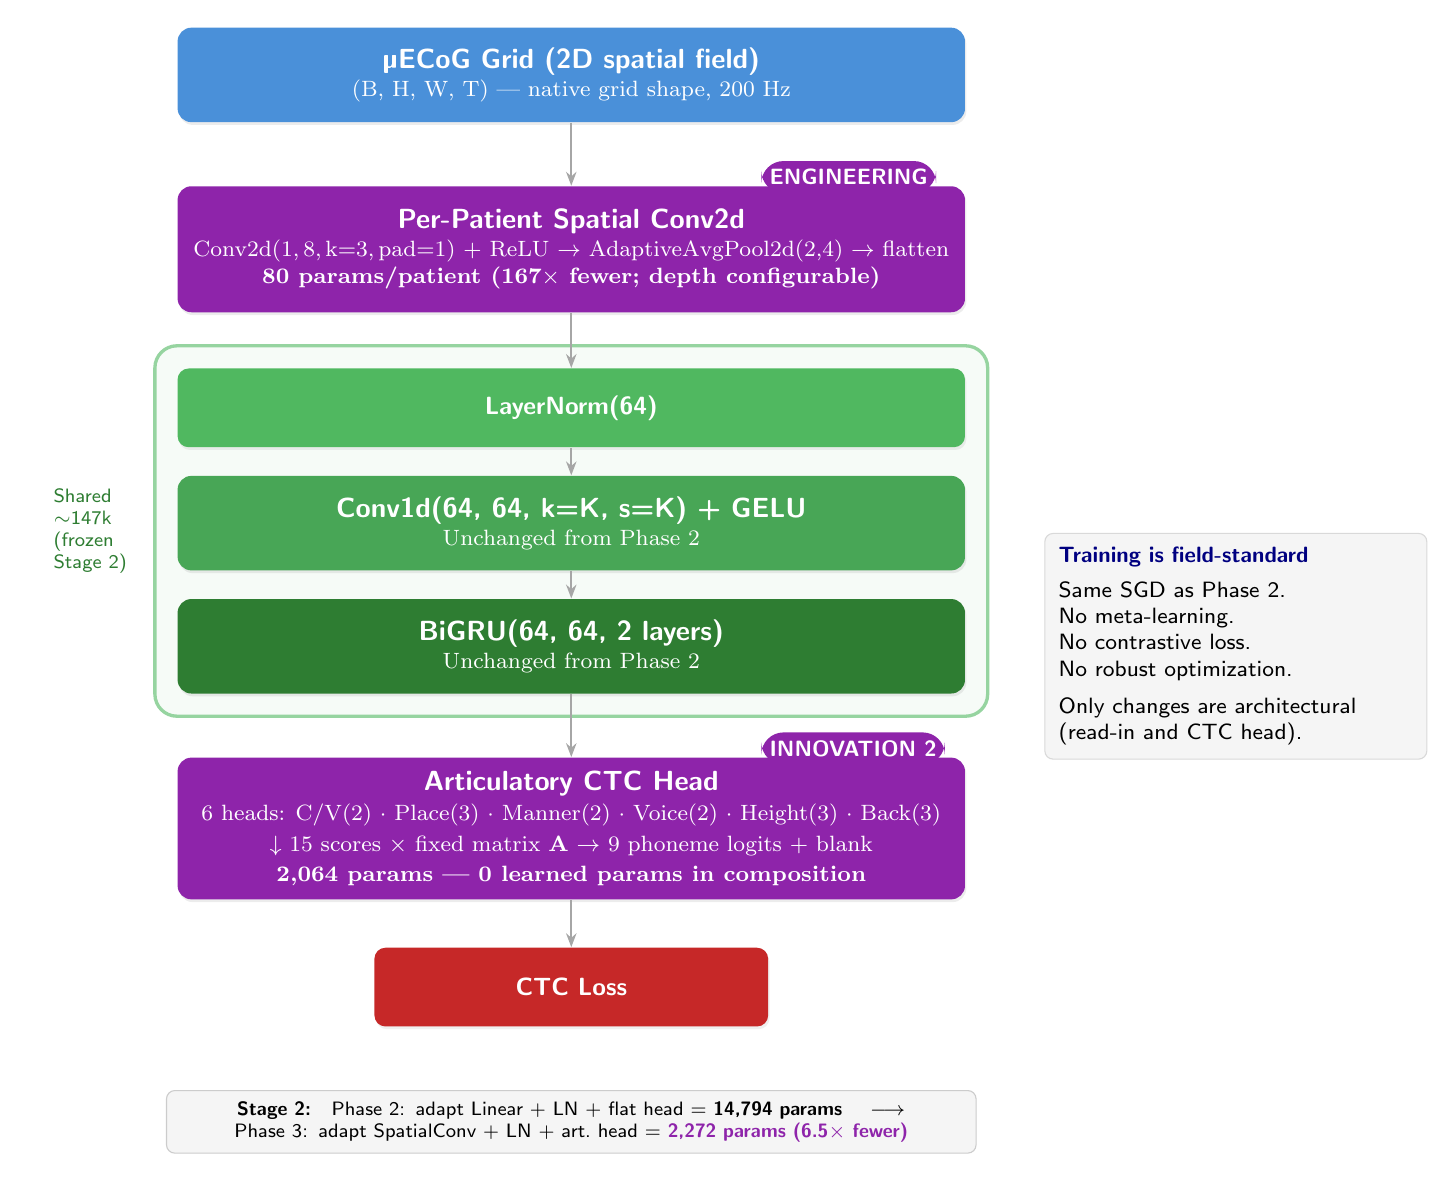
\begin{tikzpicture}[node distance=0.5cm]

  \node[block, fill=cInput, minimum width=10cm] (input)
    {\textmu ECoG Grid (2D spatial field)\\[-2pt]{\footnotesize\normalfont (B, H, W, T) --- native grid shape, 200~Hz}};

  \node[block, fill=cInnov, minimum width=10cm, minimum height=1.6cm, below=0.8cm of input] (sconv)
    {Per-Patient Spatial Conv2d\\[-2pt]
    {\footnotesize\normalfont Conv2d(1,\,8,\,k=3,\,pad=1) + ReLU $\to$ AdaptiveAvgPool2d(2,4) $\to$ flatten}\\[-2pt]
    {\footnotesize\normalfont\bfseries 80 params/patient (167$\times$ fewer; depth configurable)}};
  \node[badge=cInnov, above right=-0.1cm and -2.6cm of sconv] {\footnotesize ENGINEERING};

  \node[smallblock, fill=cShared, minimum width=10cm, below=0.7cm of sconv] (ln)
    {LayerNorm(64)};

  \node[block, fill=cShared!90!black, minimum width=10cm, below=0.35cm of ln] (conv)
    {Conv1d(64, 64, k=K, s=K) + GELU\\[-2pt]{\footnotesize\normalfont Unchanged from Phase~2}};

  \node[block, fill=cSharedDk, minimum width=10cm, below=0.35cm of conv] (gru)
    {BiGRU(64, 64, 2 layers)\\[-2pt]{\footnotesize\normalfont Unchanged from Phase~2}};

  \node[block, fill=cInnov, minimum width=10cm, minimum height=1.8cm, below=0.8cm of gru] (arthead) {
    Articulatory CTC Head\\[-1pt]
    {\footnotesize\normalfont 6 heads: C/V(2) $\cdot$ Place(3) $\cdot$ Manner(2) $\cdot$ Voice(2) $\cdot$ Height(3) $\cdot$ Back(3)}\\[-1pt]
    {\footnotesize\normalfont $\downarrow$ 15 scores $\times$ fixed matrix \textbf{A} $\to$ 9 phoneme logits + blank}\\[-1pt]
    {\footnotesize\normalfont\bfseries 2{,}064 params --- 0 learned params in composition}
  };
  \node[badge=cInnov, above right=-0.1cm and -2.6cm of arthead] {\footnotesize INNOVATION 2};

  \node[smallblock, fill=cLossDk, minimum width=5cm, below=0.6cm of arthead] (loss)
    {CTC Loss};

  \draw[arrow] (input)   -- (sconv);
  \draw[arrow] (sconv)   -- (ln);
  \draw[arrow] (ln)      -- (conv);
  \draw[arrow] (conv)    -- (gru);
  \draw[arrow] (gru)     -- (arthead);
  \draw[arrow] (arthead) -- (loss);

  \begin{scope}[on background layer]
    \node[zone=cShared!60, fill=cShared!5, fit=(ln)(conv)(gru), inner sep=8pt,
          label={[font=\sffamily\scriptsize\color{cSharedDk}]left:\begin{tabular}{l}Shared\\$\sim$147k\\(frozen\\Stage 2)\end{tabular}}] {};
  \end{scope}

  \node[annotate, fill=gray!8, draw=gray!40, text width=10cm, below=0.8cm of loss] (s2) {
    \textbf{Stage 2:}\quad
    Phase~2: adapt Linear + LN + flat head = \textbf{14{,}794 params}
    \quad$\longrightarrow$\quad
    Phase~3: adapt SpatialConv + LN + art.\ head = \textcolor{cInnov}{\textbf{2{,}272 params (6.5$\times$ fewer)}}
  };

  \node[note, right=1cm of gru] (tnote2) {
    \textcolor{NavyBlue}{\textbf{Training is field-standard}}\\[3pt]
    Same SGD as Phase~2.\\
    No meta-learning.\\
    No contrastive loss.\\
    No robust optimization.\\[4pt]
    Only changes are architectural\\
    (read-in and CTC head).
  };

\end{tikzpicture}
\caption{Phase~3 full model (E2). Purple = novel. Green = shared (frozen Stage~2). Training identical to Phase~2.}
\label{fig:phase3}
\end{figure}


% ══════════════════════════════════════════════════════════════
\clearpage
\section{The Two Innovations}
\label{sec:innovations}
% ══════════════════════════════════════════════════════════════

\subsection{Innovation 1: Per-Patient Spatial Convolution}

\textbf{Insight:} uECOG grids are 2D spatial fields---each timepoint is a low-resolution ``image'' of cortical activity. No one in the field treats them this way; everyone flattens to an unordered vector.

\begin{table}[h]
\centering\small
\begin{tabular}{@{}lcc@{}}
\toprule
& \textbf{Phase 2: Linear} & \textbf{Phase 3: Spatial Conv} \\
\midrule
Per-patient params & 13{,}376 & \textbf{80} (167$\times$ fewer; depth configurable) \\
Spatial structure & Ignored & Exploited (2D conv) \\
Grid size handling & Zero-pad to max & AdaptiveAvgPool (native) \\
Inductive bias & None & Translation equivariance \\
Stage 2 trainable & 14{,}794 & \textbf{2{,}272} (6.5$\times$ fewer) \\
\bottomrule
\end{tabular}
\end{table}

Per-patient because array orientation is \emph{not consistent} across patients---electrode (1,1) maps to different anatomical locations. Both 8$\times$16 and 12$\times$22 grids pool to $(2,4)$ transparently. Duraivel 2023: HG correlation drops below $r$=0.6 at $<$2~mm, confirming adjacent electrodes carry distinct spatial information.

\textbf{Why this matters more for uECOG than Utah:} Boccato's ``mostly diagonal'' transforms reflect Utah's fixed placement (variation $\approx$ gain). Our variable surgical placement means cross-patient variation includes spatial remapping---exactly what Conv2d's local spatial kernels capture, with far fewer parameters than a full affine matrix.

\subsection{Innovation 2: Articulatory CTC Head}

\textbf{Insight:} Motor cortex encodes articulatory gestures, not phoneme categories. Somatotopic organization maps to place of articulation (lips $\to$ tongue $\to$ larynx). Wu 2025: articulatory features ``more robustly encoded in vSMC than acoustic features.'' Duraivel 2023: confusion errors track Chomsky--Halle distance.

Six parallel sub-heads classify articulatory features:

\begin{table}[h]
\centering\small
\begin{tabular}{@{}lll@{}}
\toprule
\textbf{Head} & \textbf{Classes} & \textbf{Distinguishes} \\
\midrule
Consonant/Vowel & 2 & /b,p,v,g,k/ vs.\ /a,\ae,i,u/ \\
Place            & 3 & bilabial vs.\ labiodental vs.\ velar \\
Manner           & 2 & stop vs.\ fricative \\
Voicing          & 2 & voiced vs.\ voiceless \\
Height           & 3 & low vs.\ mid vs.\ high \\
Backness         & 3 & front vs.\ central vs.\ back \\
\bottomrule
\end{tabular}
\end{table}

15 feature scores compose into 9 phoneme logits via a \emph{fixed} binary matrix $\mathbf{A}$ (zero learned parameters in composition). Key property: /b/ vs /p/ = voicing score alone---the model \emph{must} learn voicing to distinguish them.


\subsection{Component Reference Table}

\begin{table}[h!]
\centering
\footnotesize
\setlength{\tabcolsep}{4pt}
\begin{tabular}{@{}L{2.4cm}lL{4.2cm}L{4.8cm}@{}}
\toprule
\textbf{Component} & \textbf{Status} & \textbf{Supporting papers} & \textbf{Reasoning} \\
\midrule
Per-patient input layers & Standard & Willett, Boccato, Levin, Nason, Singh, BIT & Absorbs cross-patient recording variation. Levin: shared input makes transfer worse \\[4pt]
BiGRU 2$\times$64 backbone & Standard & Singh (BiLSTM 2$\times$64, 36/44 ph), Willett/Metzger/Littlejohn (H=500--512, 50--150$\times$ data). BIT: transformer (367\,hrs) & RNNs for variable-length sequences; H=64 matches data scale. Transformers need far more data \\[4pt]
CTC loss & Standard & Willett, Metzger, Boccato, Levin, Nason, Singh (CTC). Littlejohn (RNN-T) & Alignment without frame-level labels. Universal for phoneme-level decoding \\[4pt]
Conv1d temporal downsampling & Standard & Spalding (k=10$\to$20\,Hz), Willett ($\sim$12.5\,Hz), Littlejohn (12.5\,Hz), Metzger (50\,Hz, outlier) & Most systems 12--20\,Hz. Configurable K=5 or K=10 \\[4pt]
Two-stage LOPO & Standard & Singh (Mode 3), Levin (30\% replay), Willett, Nason & Freeze backbone, adapt per-pt layers. Singh: freeze-backbone optimal \\[4pt]
LayerNorm & Standard & Chen 2024 (InstanceNorm), BIT (LayerNorm) & Per-sample; no batch stats leak. Unfrozen in Stage 2 ($\sim$128 params) \\[4pt]
Augmentation stack & Standard & Spalding ($\pm$100\,ms shift), Willett (noise), Boccato (gain dominant) & Each augmentation simulates a specific cross-patient variation source \\[4pt]
Best-checkpoint & Standard & Standard practice (no BCI paper uses SWA) & Simple; no unprecedented complexity \\
\midrule
\textbf{Per-patient Conv2d} & \textbf{Novel} & \textit{Motivated by:} Chen 2024 (3D ResNet $>$ LSTM on grids), Duraivel 2023 (HG r$<$0.6 at $<$2\,mm) & First 2D conv on uECOG. 80 vs 13{,}376 params; spatial inductive bias for remapping \\[4pt]
\textbf{Articulatory CTC head} & \textbf{Novel} & \textit{Motivated by:} Wu 2025 (articulatory $>$ acoustic in vSMC), Duraivel 2023 (errors $\propto$ artic.\ distance), Bouchard 2013 & 9-way $\to$ 6 binary/3-way sub-problems matching motor cortex encoding. Fixed composition \\
\bottomrule
\end{tabular}
\caption{Pipeline component justification. 8 of 10 components are field-standard with multi-paper support; 2 novel components are independently ablated (E3--E4).}
\label{tab:components}
\end{table}


% ══════════════════════════════════════════════════════════════
\section{What I Evaluated and Rejected}
\label{sec:rejected}
% ══════════════════════════════════════════════════════════════

Three training innovations were evaluated and downgraded to extended ablations (E5--E7):

\textbf{Reptile meta-learning.} Per-patient layers already provide transfer (Singh Mode~3). Backbone frozen in Stage~2 $\to$ ``easy to adapt'' applies to params we don't touch. $N$=7 is thin for meta-learning.

\textbf{SupCon.} CTC + per-patient layers already enforce alignment (shared head decodes all patients). Time-pooled embeddings lose sequential order. Too few positives per class.

\textbf{DRO.} Hard patients (S3: 46 trials, S5: 63 ch) are hard for \emph{practical} reasons, not neural coding differences. Upweighting = overfitting to noise. $N$=7 running EMA too noisy. Implicit difficulty-aware training already exists (higher loss $\to$ larger gradients).


% ══════════════════════════════════════════════════════════════
\section{Experiments}
\label{sec:experiments}
% ══════════════════════════════════════════════════════════════

\subsection{Core Matrix (for paper)}

\begin{table}[h]
\centering\small
\begin{tabular}{@{}lllll@{}}
\toprule
\textbf{Exp} & \textbf{Read-in} & \textbf{Training} & \textbf{CTC head} & \textbf{Tests} \\
\midrule
E0 & PCA+CCA+SVM & --- & Flat (SVM) & Baseline (0.31) \\
E1 & Linear(208,64) & Standard SGD & Flat(128$\to$10) & Field standard \\
\textbf{E2} & \textbf{Spatial Conv2d} & \textbf{Standard SGD} & \textbf{Articulatory} & \textbf{Full model} \\
E3 & Linear(208,64) & Standard SGD & Articulatory & $-$SpatialConv \\
E4 & Spatial Conv2d & Standard SGD & Flat(128$\to$10) & $-$ArtHead \\
\bottomrule
\end{tabular}
\caption{Training is identical across E1--E4. All differences are architectural.}
\end{table}

\textbf{Attribution:} E1$-$E0 = modernization gain. E2$-$E1 = innovation gain. E2$-$E3 = spatial conv contribution. E2$-$E4 = articulatory head contribution.

\textbf{Development path:} E1 $\to$ E1a (+SpatialConv) $\to$ E2 (+ArtHead). Only proceed if no PER degradation. Quick validation: 1 LOPO fold, 1 seed per step.

\textbf{Extended ablations (E5--E14):} +DRO, +Reptile, +SupCon, diagonal gain, +SWA, +DANN, +TENT, temporal dilation, pooling strategy, Conv3d hybrid.

\textbf{Evaluation:} PER primary (edit distance / 3). Balanced accuracy secondary. LOPO, 3 seeds. Wilcoxon signed-rank ($N$=8, $p<0.05$ requires $\geq$7/8 improve).


% ══════════════════════════════════════════════════════════════
\section{Data}
\label{sec:data}
% ══════════════════════════════════════════════════════════════

\begin{table}[h]
\centering\small
\begin{tabular}{@{}lllrrrl@{}}
\toprule
\textbf{Pt} & \textbf{Dx} & \textbf{Array} & \textbf{Trials} & \textbf{Sig ch} & \textbf{Frames} & \textbf{Notes} \\
\midrule
S1 & PD    & 8$\times$16  & 144 & 111 & 28{,}800 & \\
S2 & PD    & 8$\times$16  & 148 & 111 & 29{,}600 & \\
S3 & Tumor & 12$\times$22 & \textbf{46} & 149 & \textbf{9{,}200} & Fewest trials \\
S4 & PD    & 8$\times$16  & 151 & 74  & 30{,}200 & \\
S5 & PD    & 8$\times$16  & 151 & 63  & 30{,}200 & Fewest sig ch \\
S6 & Tumor & 12$\times$22 & 137 & 144 & 27{,}400 & \\
S7 & Tumor & 12$\times$22 & 141 & 171 & 28{,}200 & \\
S8 & Tumor & 12$\times$22 & 178 & 201 & 35{,}600 & Most trials/ch \\
\bottomrule
\end{tabular}
\end{table}

\begin{itemize}[nosep]
  \item Task: non-word repetition, 52 CVC/VCV tokens, 3 phonemes each (e.g., /abe/)
  \item CTC targets: 3-phoneme sequences (e.g., [a,\,b,\,e])
  \item 9 phonemes: /a/, /\ae/, /i/, /u/, /b/, /p/, /v/, /g/, /k/
  \item Paired audio: lavalier mic, MFA labels. MNI-152 coords confirmed
  \item Array orientation: NOT consistent across patients
\end{itemize}


% ══════════════════════════════════════════════════════════════
\section{Cross-Task Pooling (Duraivel 2025)}
\label{sec:crosstask}
% ══════════════════════════════════════════════════════════════

Pseudo-word repetition task with \textbf{same 9 phonemes} in CVC/VCV tokens. At least 3 patients overlap:

\begin{table}[h]
\centering\small
\begin{tabular}{@{}llrl@{}}
\toprule
\textbf{Duraivel} & \textbf{Spalding} & \textbf{Addl trials} & \textbf{Sig ch} \\
\midrule
D-S1 & S8     & 156--208 & 201/256 \\
D-S2 & S5     & 156--208 & 63/128 \\
D-S3 & S1/S2  & 156--208 & 111/128 \\
\bottomrule
\end{tabular}
\end{table}

Nearly doubles training data for overlapping patients. Same IRB, same preprocessing. Future direction (after E1--E4).

% ══════════════════════════════════════════════════════════════
\section{Questions for Zac}
\label{sec:questions}
% ══════════════════════════════════════════════════════════════

\subsection{Blocking (need before coding starts)}

\begin{enumerate}[nosep]
  \item \textbf{Where is the data?} Repo references \texttt{pt\_decoding\_data\_S62.pkl} and per-patient \texttt{.mat} files --- DABI, lab server, or elsewhere? Access process?
  \item \textbf{Patient ID mapping.} Code (S14, S23, S62\ldots) $\to$ paper (S1--S8). What's the mapping table?
  \item \textbf{Grid spatial convention.} Do \texttt{hgTrace} ch\_x/ch\_y = physical grid rows/columns? Is orientation consistent or arbitrary per patient?
  \item \textbf{Non-significant channels.} Does \texttt{hgTrace} preserve the full 2D grid with non-sig channels zeroed, or are non-sig channels excluded? Conv2d needs full grid with non-sig zeroed.
  \item \textbf{Epoch width.} Data beyond $\pm$500~ms in \texttt{.mat} files? (Need $\pm$600~ms for time-shift augmentation.)
  \item \textbf{Label encoding.} Are \texttt{phonSeqLabels} 0-indexed (0--8) or 1-indexed (1--9)? CTC blank must be index 0.
  \item \textbf{MNI coordinates and audio.} Where stored? What format? Are MFA phoneme labels already generated?
\end{enumerate}

\subsection{Important for project scope}

\begin{enumerate}[nosep, start=8]
  \item \textbf{Are there more uECOG patients?} Beyond published 8 --- others with good data (phoneme or word/nonword tasks)? Full patient list?
  \item \textbf{Which patients overlap with Duraivel 2025?} We infer D2025-S1=S8 (201/256 tumor), D2025-S2=S5 (63/128 DBS), D2025-S3=S1 or S2 (111/128 DBS). Correct? Can you disambiguate S1 vs S2?
  \item \textbf{Is pseudo-word HGA data available?} For overlapping patients --- same \texttt{.mat} format? Would we need to re-window ($\pm$1500~ms $\to$ $\pm$500~ms)?
\end{enumerate}

\subsection{Nice-to-have}

\begin{enumerate}[nosep, start=11]
  \item \textbf{Is Spalding S3 = Duraivel 2023 S4?} S3 (46 trials, 149/256 tumor) is our hardest patient. Excluded from Duraivel 2025 due to low trials? Any known bad-channel patterns?
  \item \textbf{CCA details.} Pairwise-to-universal projection method? (For baseline reproduction.)
  \item \textbf{TME surrogate.} $W$=8, $p$=0.20 had low power. Other $W$ values tried?
\end{enumerate}


% ══════════════════════════════════════════════════════════════
\section{Timeline}
\label{sec:timeline}
% ══════════════════════════════════════════════════════════════

\begin{table}[h]
\centering\small
\begin{tabular}{@{}lll@{}}
\toprule
\textbf{Phase} & \textbf{Duration} & \textbf{Depends on} \\
\midrule
Phase 0: Setup              & 1--2 weeks & Data access (Q1--2) \\
Phase 1: Reproduce baseline & 1 week     & Working code + data \\
\textbf{Phase 2: Field standard (E1)} & \textbf{2--3 weeks} & Phase 1 \\
Phase 3: Full model (E2)    & 1 week     & Phase 2 validated \\
Ablations (E3--E4)          & 1 week     & E2 converged (parallel) \\
Extended (E5--E14)          & 1--2 weeks & If time permits \\
Analysis + figures          & 1--2 weeks & All experiments done \\
\bottomrule
\end{tabular}
\end{table}

\textbf{Compute:} 4 core $\times$ 8 LOPO $\times$ 3 seeds $\times$ ${\sim}$30~min $\approx$ 48 GPU-hours.

Phase~2 is a checkpoint---publishable standalone result if Phase~3 doesn't pan out.


% ══════════════════════════════════════════════════════════════
\vfill
\begin{center}
\textcolor{gray!50}{\rule{8cm}{0.4pt}}\\[6pt]
\textcolor{gray!60}{\small Full details: \texttt{implementation\_plan.md}, \texttt{research\_synthesis.md}, \texttt{future\_directions.md}}
\end{center}

\end{document}
